%\chapter{Empirical Work}


%\chapter{Interviews with Working Professionals}
\chapter{Interviews}
\label{interviews}

This chapter discusses the conducted interviews with the working professionals.
The interviews within this research have the main purpose of helping with
identifying the problem of promotion of releases in GitOps environments,
because there is insufficient prior written literature on this topic.
Working professionals in the GitOps field are interviewed on the topic.
Their personal opinion and practical experience, use cases and concrete problems
are brought up for discussion. The importantance of a solution to the
problem is highlighted and motivated.
With the problem identification in place, several distinct solution objectives
are defined from the basis of the discussions from the interviews.
These solution objectives are then further elaborated in the following chapter
\ref{chapter:prototype}, where they primarily serve as the basis for the
desired functionality of the developed prototype.
In addition, related ideas and approaches that were discussed by the interview partners
are presented.
%Citations from interview transcripts are referred to in the following style:
%(interview 1, line 1).
The interview transcripts are found in the Appendix \ref{appendix:interview-transcriptions}.

\section{Problem Identification \& Motivation}
\label{interviews:problem-identification}

As a first step in the research process,
the overarching problem with promoting releases in GitOps environments
is elaborated in detail.
To help with this process, a series of semi-structured interviews are conducted with
practicing professionals in the GitOps field.
%In addition, prior written literature
%is also brought up to help with identification of the problem.
Furthermore, several distinct problem items are defined,
for further use in the next research activity
\ref{interviews:definitionSolutionObjectives} \nameref{interviews:definitionSolutionObjectives}.
The importance of a practical solution to the problem is highlighted.

\subsection{Problem 1: Promotion is limited to container image}
\label{problem1}

The currently available GitOps toolchains -
from e.g. Flux or Argo Projects -
provide a way to patch the newest container image version
into the desired state defined in Git.
This is offered as a plain commit without human interaction,
and is mostly used, in order to have a desired state in Git updated with
the currently latest version of a container image,
that is available in a specific container image registry.

When promoting new releases of applications or infrastructure resources defined in Git as the 
desired state, it is not only desirable to promote new version tags,
but it is also needed to promote arbitrary resources like any files
defined in the Git repository,
or Kubernetes resources, or even other external resources.
%(interview 3, line 161).

%\begin{quotation}
%	\noindent
%	\enquote*{When you're promoting, you should consider not just the image version, but all Kubernetes resources.}
%	(interview 3, line 161)
%\end{quotation}

Furthermore, it is desirable to have a human approve the changes,
which are done by a machine, e.g. with the help of Git pull requests.
The practical experience of interview partner 1 points to the idea that
very few companies really do Continuous Deployment, most of them want to have some kind of manual release.
%(interview 2, line 128).

%As interview partner 1 says:
%\enquote*{I think that very few companies really do Continuous Deployment, most of them want to have some kind of manual release.}
%(interview 2, line 128)

As interview partner 3 mentions, a release can be any combination of a general change to a system.
It should not be distinguished between a release, a hotfix, a minor or a major change.
Releases can be comprised of many changes that are new to a system,
in the Kubernetes context, this could be a new container image,
a change in a ConfigMap, or any other change in the desired state of the system.
%(interview 3, line 62).
A release may be a change to the application and or to the application specific infrastructure.
%(interview 3, line 65).
For promotion there are two important components,
the environment infrastructure, and the application itself
\autocite{gitopsAndKubernetes2021continuous}.

%Interview partner 3 defined a release
%as a \enquote*{generic change to the system}:
%
%\begin{quotation}
%	\noindent
%	\enquote*{I'm almost inclined to say that I don't care what a release is. I'm talking about a general change to the system, and whether you call it a release or a hotfix or a minor change or a major change, I wouldn't make that big of a distinction. And I wouldn't distinguish whether it's about rolling out a new container image or whether it's a change in a ConfigMap, for example.}
%	(interview 3, line 62)
%\end{quotation}

While a container image is a specific type of information inside a file in a desired state definition,
the ConfigMap stands for a generic resource, typically a separate file inside the GitOps repository.
With this statement, the interview partner means, that a release can include any type of information
or resource. When following the principles of GitOps this is usually constrained to a plain text
file in the GitOps repository, which then may be promoted by copying the file contents from
one to another GitOps environment definition.

%\begin{quotation}
%	\noindent
%	\enquote*{It's just a change to the application and or to the application specific infrastructure. So this is how I always try to explain Helm Charts or the Kubernetes Yamls.}
%	(interview 3, line 65)
%\end{quotation}

A solution to this problem could enable users to promote any arbitrary information
like a file or folder in the Git repository,
or another data from another source (e.g. artifact repository).
This is especially valuable, when thinking broadly, that the tool
which implements this problem solution, could also be used as a general
GitOps tool for interfacing with desired state definitions and moving certain
resources, or patching and updating them.

\subsection{Problem 2: Order of promotion to multiple environments}
\label{problem2}

Since currently there is no general standardized tool for promotion to multiple environments with the GitOps approach,
a specific order of promotion through environments can not easily be achieved.
For example, if an environment should only be promoted,
if the specific release has successfully passed another environment.

The desired specified order of environments could be like interview partner 3 mentioned,
where the core banking system had up to twelve environments,
%(interview 3, line 17),
which a new application release needed to pass for testing,
in a specific order.
From the practical experience of interview partner 3,
the environment setup for the critical core banking system
consisted of many environments, where the production environment with the end users,
was only a very small part.
%(interview 3, line 20).

%\begin{quotation}
%	\noindent
%	\enquote*{There have been many, many environments. Production was only a very small part of it.}
%	(interview 3, line 20)
%\end{quotation}

Due to the high criticality in the banking system,
it is the highest priority for an application to run in a stable manner throughout its lifetime,
and for new version releases and new features to not break anything.
The banking system would have a lot of environments/stages just for testing, in order to ensure the
very high quality of the software.
The criterion for an environment/stage in the context of the banking system
would be the quality level of the software.
Depending on if the software still had a lot of bugs, or it is closer to acceptance,
a new release would be in a certain environment/stage.
%(interview 3, line 26).

%\begin{quotation}
%	\noindent
%	\enquote*{The criterion for a stage was on the one hand, the quality level of the software. So does the software still have a lot of bugs, or is it close to acceptance.}
%	(interview 3, line 26)
%\end{quotation}

\begin{table}[h]
	\begin{center}
		\begin{tabular}{ |p{2.8cm}||p{1.5cm}|p{1.5cm}|p{1.5cm}|p{1.5cm}|  }
			\hline
			Tenant/Customer & A & B & C & D\\
			\hline
			Stage 1   & v1 --> v2    &v1&   v1 & v1\\
			Stage 2 &   v2  & v1 --> v2   & v1 --> v2 & v1\\
			Stage 3 &v2 & v2&  v2 & v1 --> v2 \\
			Stage 4 &v2 & v2&  v2 & v2\\
			\hline
		\end{tabular}
		\caption{Rollout to environments in stages}
		\label{table:rollout-envs-stages}
	\end{center}
\end{table}

Additionally to the order of promotion through environments,
there is the problem of rolling out new releases to all environments at once.
When
multi-tenancy is not implemented within the application,
%(interview 3, line 58),
it can be desirable to not roll out to all environments at the same time.
%(interview 3, line 158).
For example, as a platform provider with tenants represented as separate GitOps
environments, it can be desirable to split up the rollout of the new release into stages.
A new version or release could firstly be rolled out for the unimportant customer,
and after quality checks have passed,
the release could be promoted also to the important customer.
%(interview 3, line 158).
A solution to this problem formulation is especially valuable for
use cases with a high amount of regulations like e.g. financial institutions.
The rollout to environments in stages is presented in table \ref{table:rollout-envs-stages}.

%\begin{quotation}
%	\noindent
%	\enquote*{I first deployed the new version for the unimportant customer, now I also want to use it with the important customer.}
%	(interview 3, line 158)
%\end{quotation}




\subsection{Problem 3: Dependencies can not be defined}
\label{problem3}

Before promoting a new release to another environment,
it may be desirable to have specific
quality gates, which define the quality standards the
software must meet, in order to be considered for a promotion.
These can be integration, acceptance and end-to-end tests for example.
Additionally with a monitoring and observability tool,
certain metrics can be evaluated with the new release,
and if they do not meet a certain value, the release would not
be a candidate for promotion.
As a minimum, it must be ensured that the new version is 
deploying correctly. When only given the desired state definiton
in Git, it can not be measured, if the system will end up in a running
and successful deployment.

Applications may have specific dependencies to other applications or services.
%\begin{quotation}
%	\noindent
%	\enquote*{It may well be that you have dependencies between applications. I often take the approach that I have one GitOps repo per application or microservice. Now, for example, you want to promote the new version of one repo first, if the other one is also on a certain level, then there is the issue of dependencies to infrastructures, to databases, etc.}
%	(interview 3, line 155)
%\end{quotation}
To provide an example, in the context of the Kubernetes platform,
an application may need an internal service or any other external
dependency like a managed database or another infrastructure service.
%(interview 3, line 155).
When thinking of release promotion,
a dependency might be a Kubernetes object like a job or another custom resource,
which - when it is observed with a ready or successful status -
can be seen as a test result or in prinicple a quality gate, which qualifies the
new application release for promotion.

A solution to this problem statement is especially valuable when having the whole
continuous delivery lifecycle in mind. After deployment of a new application release
to a certain environment, it should be evaluated for its quality. So, tests
and other metrics should be evaluated, in order to ensure high software quality
at every stage in the development and also deployment cycle,
all this in a fully automated way.

\subsection{Problem 4: Provider and tool dependency}
\label{problem4}

With the currently available GitOps toolchains,
and due to the lack of best practices and standardized solutions,
users or platform engineers are inclined to build
and setup
advanced and complex pipelines that are interdependent on a lot of things,
as interview partner 1 highlights.
%(interview 1, line 311)
This usually results in tight coupling of the Git provider, the GitOps engine, the CI workflow/pipeline platform,
configuration management tools, and other components.
Since many tools in the GitOps ecosystem are not very mature in their development and adoption,
it is of use that components are loosely coupled and can be exchanged with alternatives in the future.
Additionally there need to be permissions and policies granted to many different people and
machines on many different systems.
In the end, it results in vendor lock-in and tightly coupled toolchains.

A solution to this problem enables users to avoid vendor lock-in as much as possible.
This fits well with the Kubernetes ecosystem, which is currently the most prominent
cloud native software platform,
in that it also tries to be cloud and platform agnostic at every step of the way.
With Kubernetes it is always desirable that applications running on the platform can
run on any type of infrastructure.











\section{Definition of Solution Objectives}\label{interviews:definitionSolutionObjectives}

Now that the problem has been identified in the earlier section
\ref{interviews:problem-identification} \nameref{interviews:problem-identification},
research objectives of a solution to the problem will be inferred.
Each objective provides a solution to a distinct problem item
(fig. \ref{fig:from-problem-to-objective-visualized}).

\begin{figure}[h]
	\centering
	\fbox{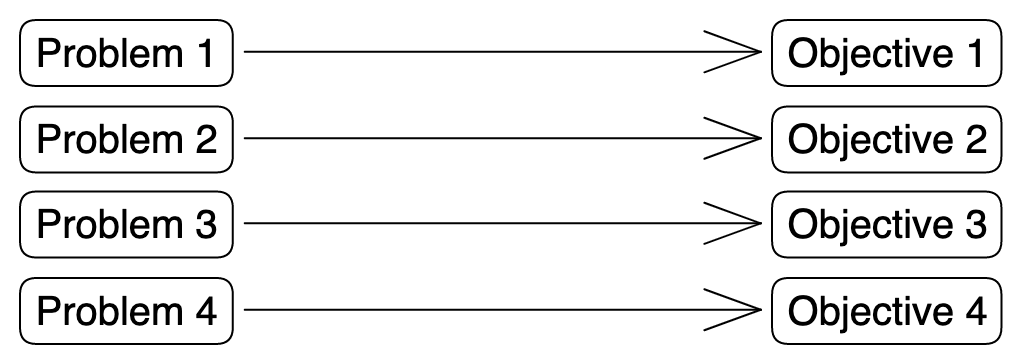
\includegraphics[width=0.55\linewidth]{assets/from-problem-to-objective-visualized.png}}
	\caption{Definition of Solution Objectives by inferring from Problem Definitions.
		%		(\citeauthor{ref}, \citeyear{ref}).
	}
	\label{fig:from-problem-to-objective-visualized}	
\end{figure}

A solution objective is a qualitative description of how the functionality
of the developed prototype is expected to support a solution to the problem definition.
For later evaluation of the results, the observed functionality can be backtracked to
a certain solution objective and its respective problem item.

\subsection{Objective 1: Arbitrary resources can be promoted}
\label{objective1}

From the problem definition
\textit{\nameref{problem1}},
a solution objective
\textit{\nameref{objective1}},
is inferred.
A qualitative description of the solution objective
is pointed out in the following.

A promotion subject, which is promoted between GitOps environments can potentially
be of many types. A popular type of data, which can be promoted,
is the version tag of the container image of a particular application.
For some use cases it is not sufficient to promote only the version of the container image.
In order to provide a solution to this problem,
the solution must provide a way to promote arbitrary types of resources.
In the GitOps context, resources are typically constrained to declarative
representations in plain text format, which are defined in a Git repository.
By providing a way to copy user defined files or directories in the form
of filesystem paths inside a Git repository,
potentially any type of resource may be a possible subject for promotion.
When GitOps environments are stored in multiple, separate Git repositories,
there needs to be the functionality to copy between these repositories.
This is illustrated in figure \ref{fig:OBJ1R1-and-OBJ1R2}.
%

\begin{figure}[h]
	\centering
	\fbox{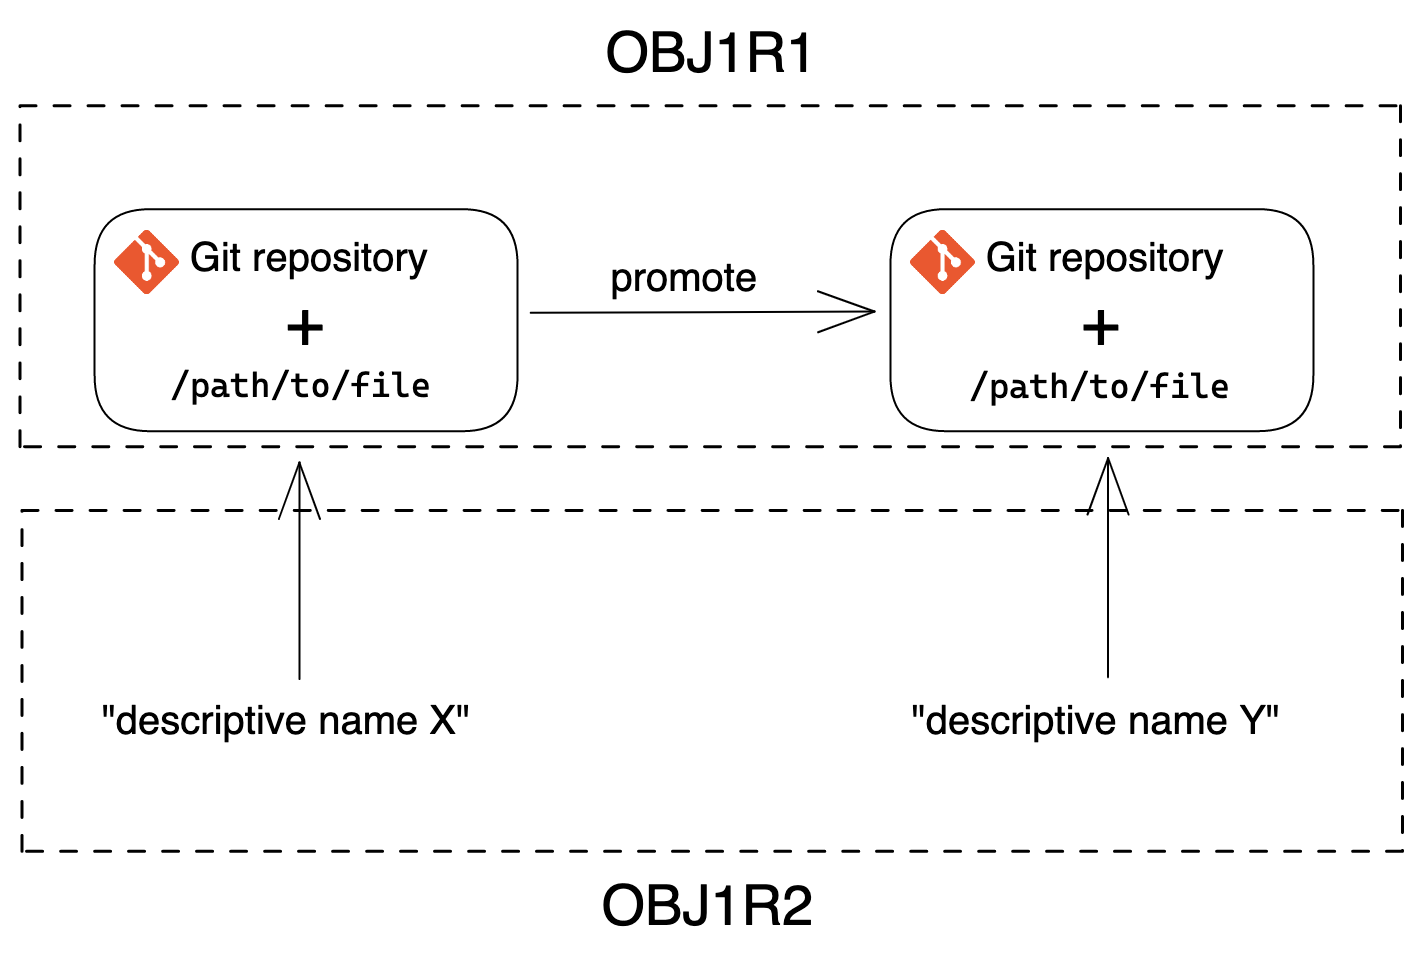
\includegraphics[width=0.79\linewidth]{assets/OBJ1R1-and-OBJ1R2.png}}
	\caption{\nameref{objective1}.
		%		(\citeauthor{ref}, \citeyear{ref}).
	}
	\label{fig:OBJ1R1-and-OBJ1R2}	
\end{figure}

Furthermore, for these arbitrary files or directories in GitOps repositories
a descriptive name for a certain file or directory
should be defined alongside the
respective copy operation of the promotion subject.
This is useful for identifying the specific promotion subject
on a higher abstract level.
This way, for example, an application's environment variables,
which are defined and actually disguised as a Kustomize overlay in a Kubernetes deployment resource,
can be given a friendly name like "Environment variables/Application Configuration".
This makes it a lot easier to identify a particular promotion subject, without
needing to manually inspect the raw contents of a file or even multiple files or
directory trees.
This is illustrated in figure \ref{fig:OBJ1R1-and-OBJ1R2}.

A collection of the requirements for the solution objective is shown below
Each requirement is represented in the form of a user story
\autocite{userStoriesCohn2004user},
and is labelled with a code, from a combination of the
objective's code (e.g. OBJ1) and the requirement's code (e.g. R1).

\begin{itemize}
	\item OBJ1R1: \setword{As a user, I can define any filesystem path inside a Git repository, with a respective target path in a Git repository, as a promotion subject.}{OBJ1R1}
	\item OBJ1R2: \setword{As a user, I can define a descriptive name for a promotion subject, which is represented as an arbitrary filesystem path.}{OBJ1R2}
\end{itemize}

These requirements are formulated from the perspective of the user of the developed prototype.
Not exclusively the user can evaluate whether the requirement is fulfilled.
An observer, like the researcher, can evaluate the fulfillment of a solution objective
on the basis of the demonstration (section \ref{prototype:demonstration}).

\subsection{Objective 2: Strict flow of promotion through environments}
\label{objective2}

From the problem definition
\textit{\nameref{problem2}},
a solution objective
\textit{\nameref{objective2}},
is inferred.
A qualitative description of the solution objective
is pointed out in the following.

When promoting a new application release to multiple environments,
it may be necessary to define a certain order, in which the promotion proceeds
through the environments (fig. \ref{fig:OBJ2R1}).
This can have many reasons,
as defined in the problem identification section \ref{problem2} earlier.
A release may be rolled out to the initial development environment continuously,
without any quality gates or other checks, to ensure software code and runtime quality.
However, in order for a new version release to proceed to environments like
performance test environments, which can produce high resource costs for each test,
it may be useful to control the deployment to certain environments and this way, further constrain
the deployment to subsequent environments, with a step in between.
Another use case for this solution objective is for service providers
with a multi-tenant architecture, which is implemented with GitOps environments.
These service or platform providers may want to rollout a new release with a certain staging process.

\begin{figure}[h]
	\centering
	\fbox{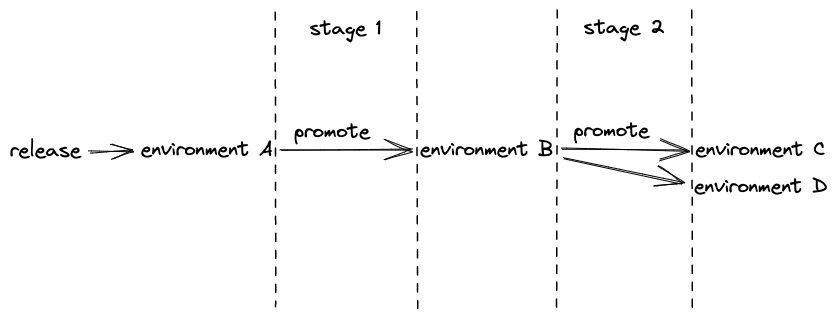
\includegraphics[width=1.00\linewidth]{assets/OBJ2R1.png}}
	\caption{\nameref{objective2}.
		%		(\citeauthor{ref}, \citeyear{ref}).
	}
	\label{fig:OBJ2R1}	
\end{figure}

A collection of the requirements for the solution objective is shown below.
Each requirement is represented in the form of a user story,
and is labelled with a code, from a combination of the
objective's code (e.g. OBJ2) and the requirement's code (e.g. R1).

\begin{itemize}
	\item OBJ2R1: \setword{As a user, I can promote releases through multiple environments in a certain user-defined order.}{OBJ2R1}
%	\item \textbf{OBJ2R2}: \setword{As a user, I can rollout a release to specific environments, while leaving others untouched.}{OBJ2R2}
\end{itemize}

The initial release to the first environment (environment A in figure \ref{fig:OBJ2R1})
is not handled by the developed operator prototype.
However, the subsequent stages (stages 1 and 2 in figure \ref{fig:OBJ2R1})
are automated by the promotions operator.

\subsection{Objective 3: Dependencies of a promotion}
\label{objective3}

From the problem definition
\textit{\nameref{problem3}},
a solution objective
\textit{\nameref{objective3}},
is inferred.
A qualitative description of the solution objective
is pointed out in the following.

After deploying a new release to a certain environment,
the minimum requirement for further proceeding to a subsequent deployment environment,
is typically to check if the application was deployed successfully and is running in a healthy state.
While this is the minimum that should always be ensured before promotion,
other types of processes may be done, in order to reduce the likelihood of delivering bad quality software,
which could likely be introduced by a bad release.
One of these can be to have dependencies for a promotion.
In the context of Kubernetes, this could be another Kubernetes workload, or any other object or custom resource.
Kubernetes native testing tools or workflow engines may provide custom resources with Kubernetes API conformant
conditions, in order for other programs to check the state of the resource, in particular this may be the ready condition.
This solution objective is illustrated in figure \ref{fig:OBJ3R1}.

\begin{figure}[h]
	\centering
	\fbox{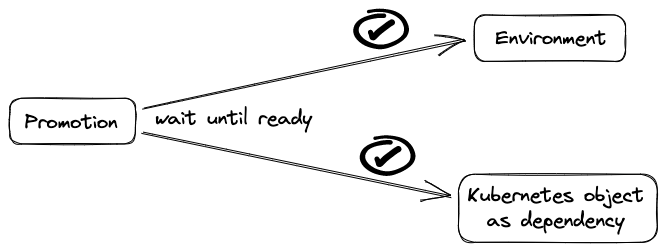
\includegraphics[width=0.82\linewidth]{assets/OBJ3R1.png}}
	\caption{\nameref{objective3}.
		%		(\citeauthor{ref}, \citeyear{ref}).
	}
	\label{fig:OBJ3R1}	
\end{figure}

A collection of the requirements for the solution objective is shown below
Each requirement is represented in the form of a user story,
and is labelled with a code, from a combination of the
objective's code (e.g. OBJ3) and the requirement's code (e.g. R1).

\begin{itemize}
	\item OBJ3R1: \setword{As a user, I can define Kubernetes objects as dependencies for a promotion.}{OBJ3R1}
\end{itemize}

A promotion process can have predefined dependencies, which must be ready or successful
before a promotion is triggered.
The prototype design sees a Kubernetes object as a dependency. This can be a certain
workload like a deployment, a test run, a database, or any other object/resource.
The environment (in fig. \ref{fig:OBJ3R1}) is the aggregation of all resources
that are defined in the respective desired state in the GitOps repository.

\subsection{Objective 4: Vendor-neutral, tool-agnostic}
\label{objective4}

From the problem definition
\textit{\nameref{problem4}},
a solution objective
\textit{\nameref{objective4}},
is inferred.
A qualitative description of the solution objective
is pointed out in the following.

\begin{figure}[h]
	\centering
	\fbox{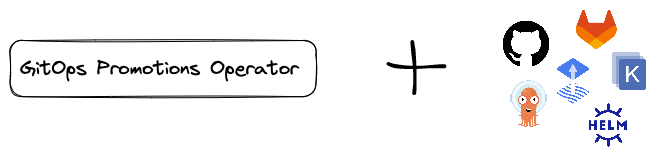
\includegraphics[width=0.80\linewidth]{assets/OBJ4R1.png}}
	\caption{\nameref{objective4}.
		%		(\citeauthor{ref}, \citeyear{ref}).
	}
	\label{fig:OBJ4R1}	
\end{figure}

When following current good practices and guidelines
to build a promotion setup for GitOps environments,
users are inclined to build workflows which are constrained to specific Git providers, GitOps engines,
CI pipeline and configuration tools. This leads to tightly coupled setups,
and vendor lock-in.
With the strong open-source foundation of the Kubernetes platform and ecosystem,
it is a good practice to build additional tools and platforms on top of Kubernetes,
in order to remain cloud and vendor agnostic. In the space of GitOps promotions,
there is currently insufficient tooling for this purpose.
Therefore, one solution objective of this research (fig. \ref{fig:OBJ4R1}) is to
provide a generic tool,
which is vendor-neutral,
and agnostic to the Git provider, as well as the configuration/templating tool.

A collection of the requirements for the solution objective is shown below
Each requirement is represented in the form of a user story,
and is labelled with a code, from a combination of the
objective's code (e.g. OBJ4) and the requirement's code (e.g. R1).

\begin{itemize}
	\item OBJ4R1: \setword{As a user, I can use any GitOps engine, Git provider and configuration/templating tool.}{OBJ4R1}
\end{itemize}

The developed prototype operator is compatible with all GitOps engines
like Flux or ArgoCD, configuration tools like Helm or Kustomize,
Git providers like GitHub or GitLab.
The primary purpose of this vendor-neutrality trait is to
have a wider pool of potential users who can give early feedback.
An integration to certain tools can be built in the future, in order to enhance the user experience and ease of use.






\section{Insights into Related Ideas and Approaches}
\label{insights-related-ideas-approaches}

The conducted semi-structured interviews gave valuable insights into
the unique views on the problem and related topics of each of the working professionals.
Some of the related ideas and alternative approaches are discussed in this section.

\subsection{Rolling Production Environments}

Interview partner 1 mentioned a new idea of
rolling production environments.
%(interview 1, line 221).
With this approach,
on major changes a new production environment would be created,
and then progressive delivery would be done against the whole environment.
This includes the application and the whole infrastructure layer below it.
In the Kubernetes context this would be the cluster itself, not only the deployment resource.
%(interview 1, line 221).
%It was defined like the following:
%\enquote*{if we have major changes instead of doing progressive delivery on an application level, how about just setting up a new production environment and then start doing progressive delivery against the new cluster}
%(interview 1, line 221).
%\enquote*{Why not just set up a new cluster since it's GitOps, We can just you know, we we have environment creation automated, we have everything stored in Git.}
%(interview 1, line 224)
Since GitOps allows to easily recreate the whole environment infrastructure,
this is not difficult to achieve.
With tools like the GitOps Terraform Controller
\nolinebreak
\footnote{https://github.com/weaveworks/tf-controller}
such a setup is easier to achieve than before, without the GitOps approach.
%(interview 1, line 224).

%\enquote*{So at some point we're going to have progressive delivery, not on a specific application, but more of on entire environments.}
%(interview 1, line 227)

Interview partner 1 discussed this idea as an alternative to having different long-living environments,
what would have been done in the past.
Instead, the idea is to re-create entire copies of the production environment,
with the power of GitOps,
and do progressive delivery for that copy of the environment as a whole.
%\enquote*{cloud, native is immutable infrastructure. So why shouldn't the platform also be immutable?}
Not only the application - the running container - but also the platform and infrastructure below
can be immutable and versioned.
%(interview 1, line 251).
This could be done, in order to further limit the impact of a bad change in a new release of the software version.
In addition, when having not just the desired state of the application, but also the entire infrastructure below it,
stored in Git,
it also increases the immutability and therefore resiliency of the user-facing service.

In the Kubernetes ecosystem, there have emerged a lot of applications,
which are providing certain services like the Cert-Manager and TLS certificates,
or services which are providing policy functionality.
These applications responsible for infrastructure or for supporting the primary application,
which is in the end user-facing,
all have their own version and are constantly updated.
There is also the possibility that a new release of such a supporting service
can break the primary user-facing application.
%\enquote*{So there's applications there, etc., etc., etc. before we even get to the part that is our particular code, we have like 20 different applications that are backing up this system and they change versions, our code changes versions, Kubernetes is upgraded and stuff might be deprecated or even removed. Doing that as the environment is actually running is what kind of makes people sweat.}
%(interview 1, line 239)
Kubernetes deployments might have many different applications,
which are providing supporting services for the actual custom application.
All these might be critical dependencies. Every dependent service can change version,
Kubernetes itself is upgraded, and some APIs might even be deprecated or removed.
There are many variables that could cause an outage of the particular critical user-facing service.
%(interview 1, line 239).
%\enquote*{This is that's why you have the maintenance windows where people are staring at the clusters doing upgrades and things like that. Well, for me it just makes so much more sense. Just putting up an entirely new environment with all new versions and our new production, you know, code. Does it work? Cool. All right, Point DNS towards new cluster and you're done, right?}
%(interview 1, line 242)
Usually there would be a maintenance window for major new version releases,
where responsible people are ready, incase anything breaks during a new release.
The chance of failures could be decreased with this new approach,
where the entire production environment is replaced with all new components with new versions.
%(interview 1, line 242).
%\enquote*{So there's no downtime for users even. [...] So that is I think the end goal for us when it comes to how we do promotions and getting new code out there.}
%(interview 1, line 245)
Interview partner 1 sees this idea of rolling production environments as one of the next steps to move towards with the GitOps approach.
%(interview 1, line 245).

%When asked if this idea is related to or could be called blue-green deployments:
%\enquote*{So I would rather not call it blue green and rather have a new term for it.}
%(interview 1, line 257)

\subsection{Overview of GitOps Repositories}

Interview partner 2 discussed the idea, that
currently when using common tooling,
it can be quite cumbersome to get a grip of what is inside a GitOps repository/environment,
just by looking at the filesystem tree and plain text files.
GitOps tools like Argo can visualize the other way around,
meaning the ArgoCD dashboard can visualize what is deployed by ArgoCD itself
in a specific deployment environment, i.e. cluster or namespace.
However, when a human looks at the plain GitOps repository,
it can be difficult to understand the setup.
So the advantage of GitOps having a single source of truth,
where the human operator or developer can look,
and understand at one glance what the truth is,
is kind of lacking at the moment with the current ecosystem of GitOps tools.
%\enquote*{The nice overview that GitOps is supposed to bring in theory, where I can say, ok I have a single place where I look in, which for me is already a big advantage of the whole approach, I lose it a bit, you always have to look at different places to know what is deployed there, the overview is missing a bit.}
%(interview 2, line 113)
The good overview that GitOps is supposed to bring in theory
- when thinking of the aspect of the desired state being the single source of truth, with declarative configuration that is easy to read -
seems to be a bit insufficient at the moment with the currently available tools.
%(interview 2, line 113).

%\enquote*{That's something that I find a bit unattractive currently with GitOps.}
%(interview 2, line 116)
%
%\enquote*{I don't think there is a great solution at the moment.}
%(interview 2, line 119)

What goes hand in hand with this topic of the overview over GitOps repositories
is the overview of versions that are deployed,
and where the versions are deployed.
With a GitOps setup, there are a couple of versions, or revisions, for different sources.
There is often a version of the GitOps repository, the Helm or Kustomize reference or many of those,
and the different container image versions.
With all these different versions at different places,
it can be confusing.
A better overview over the deployed versions of a GitOps repository
would be good to have.
%(interview 2, line 104).
It might not be desirable to know the revision of the GitOps repository,
where the desired state is stored,
but better to know the version of the Helm or Kustomize configuration that is stored in the repository.
%(interview 2, line 107).

%Interview partner 2:
%
%\enquote*{You have a lot of versions, and that makes it very confusing. And often it's not clear which version you have now and with Argo CD, for example, that's still not well solved because you have revision, but the revision is actually the revision of the configuration and not the version of the Helm or Kustomize, which is what I would actually want.}
%(interview 2, line 104)
%
%\enquote*{Because I want to know what revision of helm or Kustomize is in there and not the revision of the config repo, which is actually just the composition of the versions that are deployed.}
%(interview 2, line 107)
















\section{Summary}

This chapter discussed the problem identification and motivation of the main topic of this thesis,
namely the promotion of releases in GitOps environments.
With the help of practicing professionals, who are working in the GitOps field,
several problems have been identified,
and defined along with research objectives which should provide a possible solution.

\nameref{problem1},
relates to a frequent issue with currently available tooling in the GitOps ecosystem. 
Often times solely container image version tags are the focus with current tools when promoting
new versions or releases. It was discussed, that this is insufficient for some use cases.
It is sometimes required to handle all sorts of resources, not just the version tag of a container image.
Especially when not using containerization technologies for runtime, this is an important problem to handle.
In order to be able to provide a solution to this problem with a comprehensible approach,
a solution objective was inferred and its requirements defined.

\nameref{objective1},
defines a qualitative description of how the respective problem is supposed to be solved
by the developed artifact. The main idea is to offer the capability to promote arbitrary resources,
meaning any type of resource, instead of solely the container image version.
The technical implementation in the proposed prototype foresees the functionality for
promoting a list of filesystem paths inside the Git repository of the desired state to other environments.
In addition these arbitrary resources should be able to be assigned a descriptive name,
in order to identify the promotion subjects more easily.

\nameref{problem2},
states the fact, that it is not a straight-forward process of how the order of promotion
through multiple GitOps environments can be setup. When adhering to the principles of GitOps
and the asynchronous deployment process (described in chapter \ref{theoretical-background})
there is no streamlined approach or tooling, that automates this.

\nameref{objective2},
defines the requirements for the proposed prototype,
in regards to the according problem of having a certain order of promotion through environments or stages.
The objective describes the capability for defining a certain order of environments, in which releases traverse through.
In addition, this solution objective opens up the possibility to setup promotion in stages, in which
certain environments must be deployed to first, before the release can deploy to other specified environments.

\nameref{problem3},
relates to the problem that when wanting to promote a new release from one environment to another environment,
it is not easily achievable with the available tools to specify certain dependencies, like other workloads or
microservices in the same or another environment, or altogether dependencies from external sources.
This is especially desirable for evaluating test results or other metrics, before triggering the promotion.

\nameref{objective3},
describes how the respective problem of being able to specify dependencies for a promotion,
could be solved in the proposed prototype. While the minimum dependency is the successful deployment
of the workload of a release,
it may also be desirable to specify other resources or workloads which need to be in a certain state,
before triggering a promotion.

\nameref{problem4},
draws attention to the common problem of being dependent on single tools and providers.
The more complex the Continuous Delivery is setup for a particular project,
the more difficult it is to de-couple or switch providers for certain components.
Furthermore, since many tools in the GitOps ecosystem are not very mature in their development and adoption,
it is of use that components are loosely coupled and can be exchanged with alternatives in the future.

\nameref{objective4},
defines the requirements of how a vendor-neutral and tool-agnostic prototype can be implemented.
The main components which are desirable to support all alternatives,
for being able to switch between them,
are the Git providers (e.g. GitHub, GitLab),
the GitOps engines (e.g. Argo, Flux),
the configuration/templating tools (e.g. Kustomize, Helm).

Additionally,
related ideas and approaches were discussed by the interview partners.
These points were not directly considered for the conducted design science in the prototype,
however they are discussed later in chapter \ref{discussion-and-interpretation}.
















\chapter{Prototype}
\label{chapter:prototype}

This chapter describes the developed prototype,
called the \textit{GitOps Promotions Operator}.
First, the asynchronous nature of a typical GitOps deployment is described,
and where the proposed \textit{GitOps Promotions Operator} prototype finds its place within
this architecture.
Next, abstract models and their respective custom resources are designed which describe the \textit{Environment} and \textit{Promotion} 
custom resources; which are then afterwards implemented as mockups of 
Kubernetes custom resources in the declarative Yaml specification syntax.
Next to the mockups implemented in the prototype,
additional alternative mockups are suggested for possible alternative implementations.
Then, the implementation of the custom resource definitions and respective controller logic
is described within the context of the used Kubernetes operator framework Kubebuilder.
Once the design and development of the artifact - the \textit{GitOps Promotions Operator} prototype -
is successfully done,
the operator is demonstrated in a proof of concept,
and finally evaluated against the solution objectives
from section \ref{interviews:definitionSolutionObjectives}.

\section{Design \& Development}

The design and development of the prototype
is based on the research objectives defined in section
\ref{interviews:definitionSolutionObjectives}.
The overarching goal is to fulfill the objectives with the developed artifact,
the \textit{GitOps Promotions Operator} prototype.
This is shown by demonstrating the functionality and evaluating against the research objectives.

\subsection{Asynchronous GitOps Deployments}
\label{prototype:design:async-gitops-deployments}

First, the process of a typical GitOps deployment needs to be addressed, where
the proposed \textit{GitOps Promotions Operator} prototype needs to find its place in this asynchronous process.

\begin{figure}[h]
	\centering
	\fbox{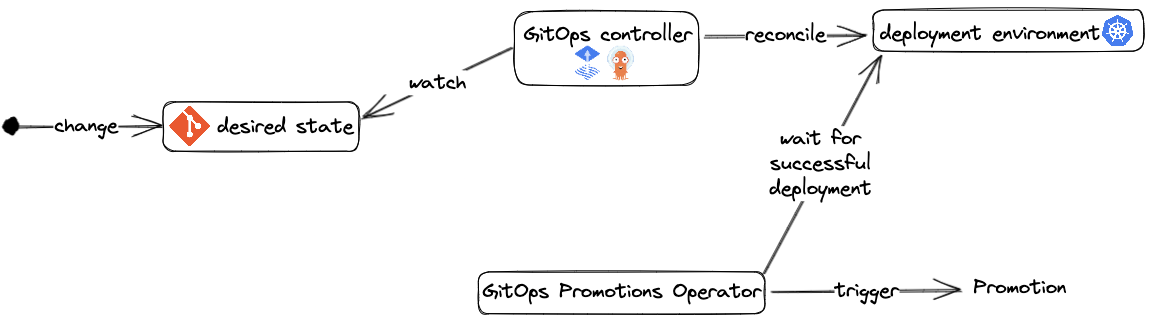
\includegraphics[width=0.98\linewidth]{assets/async-gitops-promo-arch.png}}
	\caption{Asynchronous GitOps deployment and promotion.
		%		(\citeauthor{ref}, \citeyear{ref}).
	}
	\label{fig:async-gitops-promo-arch}	
\end{figure}

It begins with a change of the declarative state definitions in a Git repository,
which is then being reconciled by the GitOps controller.
The timeframe from the change of the desired state to the actual state being applied
is variable. An external system (i.e. the \textit{GitOps Promotions Operator}), which watches the desired state, has no knowledge of
the current state of the deployment environment - when solely given the desired state in the
Git repository. An external system also does not know whether the desired state works or not
(e.g. when the new version fails to rollout).

The proposed \textit{GitOps Promotions Operator} ideally needs to pick up
the asynchronous deployment process after the new release of the desired state
has been successfully rolled out to the deployment environment.
In order to achieve this,
it needs to at least check the availability of the deployed application or workload,
before continuing on with the promotion.
The described asynchronous GitOps deployment and promotion model can be seen in figure
\ref{fig:async-gitops-promo-arch}.

In order for the proposed \textit{GitOps Promotions Operator} prototype to fit into
this asynchronous deployment architecture,
it needs to have several asynchronous phases in its controller logic.
The minimum steps or phases it needs are the following:

\begin{figure}[h]
	\centering
	\fboxsep6mm\fbox{\begin{tikzpicture}[node distance=1.3cm]
		\node (start) [startstop] {Start};
		\node (one) [process, below of=start] {watch deployment environment};
		\node (two) [process, below of=one] {wait for successful deployment};
		\node (three) [process, below of=two] {trigger promotion};
		\node (stop) [startstop, below of=three] {Stop};
		
		\draw [arrow] (start) -- (one);
		\draw [arrow] (one) -- (two);
		\draw [arrow] (two) -- (three);
		\draw [arrow] (three) -- (stop);
	\end{tikzpicture}}
	\caption{Asynchronous Phases of Deployment.} \label{tikz:async-phases-deploy}
\end{figure}


In order to check if a deployment was successful,
the \textit{GitOps Promotions Operator} needs access to the deployment environment. This is already given,
if the operator is running inside the same deployment environment.
For the promotion process, the operator also needs access
to the source and the target
environment (Git repository).
The described architecture can be viewed in figure \ref{fig:operator-access-source-target-envs}.

\begin{figure}[h]
	\centering
	\fbox{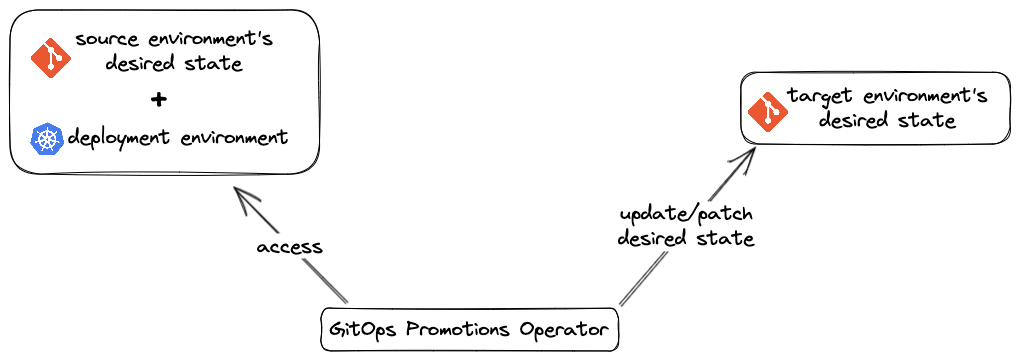
\includegraphics[width=0.98\linewidth]{assets/operator-access-source-target-envs.png}}
	\caption{GitOps Promotions Operator Promotion from source to target environment.
		%		(\citeauthor{ref}, \citeyear{ref}).
	}
	\label{fig:operator-access-source-target-envs}	
\end{figure}

%\subsection{old intro.....}
%
%The \textit{GitOps Promotions Operator} prototype
%is implemented with the Kubebuilder framework,
%discussed in section \ref{theoretical-background:kubernetes} of this thesis.
%The main constraints the framework comes with, are the
%custom resource definition + controller pattern.
%
%\begin{figure}[h]
%	\centering
%	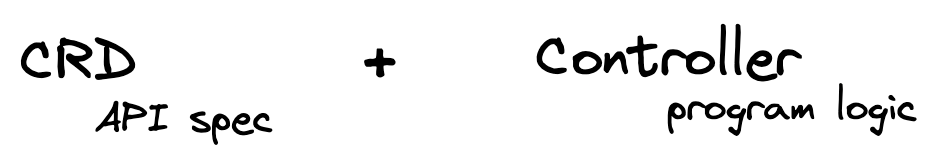
\includegraphics[width=1.00\linewidth]{assets/crd-and-controller.png}
%	\caption{Custom Resource Definition and Controller.
%		%		(\citeauthor{ref}, \citeyear{ref}).
%	}
%	\label{fig:crd-and-controller}	
%\end{figure}
%
%As the initial step of the design phase,
%abstract model definitions are designed.
%Their key properties are identified.
%Then a sample mockup is designed as
%a custom resource definition in Yaml format.
%Afterwards this idea of the model definition is 
%translated into custom struct types of the
%Go programming language,
%which is chosen by the Kubebuilder framework.

Once the architecture of the asynchronous GitOps deployment process,
and where the \textit{GitOps Promotions Operator} fits within this process is clear,
the abstract models for the custom resources and their functionality can be designed.






\subsection{Abstract Models}
\label{prototype:design:abstract-models}

In this section,
abstract models for environments, as well as promotions are designed.
The term abstract model stands for a qualitative description of a resource.
The abstract model is supposed to function as a high level abstract representation of a resource,
that exists in the actual world, either internal or external to the system,
or is used purely as an abstraction layer for such an actual resource.

\subsubsection*{Environment Model}

In the context of this software prototype,
an environment is a GitOps environment as defined in section
\ref{theoretical-background:gitops}.
As a reminder, this is a folder/directory in a Git repository,
which essentially points to a deployment environment, typically being a Kubernetes cluster/namespace.
Therefore, the model for the environment primarily represents a directory path in a certain Git repository.
This can potentially be a specific branch or any commit or refspec
\nolinebreak
\footnote{https://git-scm.com/book/en/v2/Git-Internals-The-Refspec}
in the Git repository.

In addition to the Git repository and the path pointing to the GitOps environment,
the abstract model has a definition of dependent resources inside the deployment environment.
This is needed in order for the operator to know which resources are deployed and belong to the desired state definition;
and furthermore to achieve the possibility to define dependencies,
which need to be fulfilled before a promotion is allowed to be triggered.
A dependency can be potentially anything, which needs to be in a certain state, before a promotion is triggered.
Abstract examples of dependencies could be e.g.
HTTP(S) endpoints internal or external to the deployment environment which return a certain response;
Kubernetes objects which need to have a certain condition or be in a certain state.

As an alternative to a Git repository,
the desired state of the GitOps environment could also be stored in a object store elsewhere
like an object or blob store or an artifact registry;
or it could be stored in an alternative version control system, other than Git.
The desired state could also be a combination of these possible sources.
The described other possiblities for the desired state store are not further handled in the proposed prototype,
however they must be noted and considered in the base architecture, in order for the possibility to support
them in the future.

\subsubsection*{Promotion Model}

In the context of this software prototype,
a promotion is a GitOps promotion as defined in section
\ref{theoretical-background:gitops}.
As a reminder, this is the process of promoting a new application or infrastructure version
to another deployment environment, which typically means a change in the desired state definition in a GitOps environment.

For the proposed and implemented prototype within this concrete research,
the process of a GitOps promotion is the change of the desired state definition of a certain GitOps environment,
typically mentioned as the target environment of a promotion. For the prototype,
the declarative state, which is promoted, i.e. changed in the target environment, is drawn from the
source environment's desired state definition. In the easiest case, this means that a certain
file or directory is copied from the source to the target environment - or a list of files/directories.
These files or directories which are promoted, are called promotion subjects within the context of this
thesis.

Promotion subjects can potentially be of many other types, however other types are not implemented in the prototype.
Examples for other promotion subjects could be other representations of resources in the desired state,
like object references to Kubernetes built-in resources or custom resources instead of plain text files or directories.
Custom resources could be ArgoCD Applications or other high-level abstractions or collections of resources.
As alternative sources for promotion subjects,
the operator could gather other arbitrary information. For example this could be information like a version tag
of an artifact repository.
This arbitrary data point could then be patched statically in a certain YAML path of a file.
Alternatively, it could be patched into lines, which have been marked as comments in files in advance.
The mentioned strategies are used by other software programs, which interface with plain text desired state definitions.

What should also be mentioned, but is not implemented in the proposed prototype,
is that a promotion process could be of other types.
As an example, this could be the difference between two commits of Git repositories,
which is essentially a patch between two states. This difference could be applied to another environment.

The promotion process could possibly have hooks or phases before and afterwards, which could be configurable by the user.
Furthermore, such a promotions operator could have the functionality to combine multiple promotions together.
This way, the end-to-end observability and manageability would be improved.
This is in line with a problem discussed earlier, of the overview over GitOps environments
and the deployed applications. On top of that, a functionality could be developed
to increase observability into e.g. the current state of a specific release and which environments it passed.

Another alternative possibility of a promotion process or how a promotion could be achieved,
is that Git branches are leveraged.
This could mean, that an environment would differ from another environment just by the branch of the same Git repository.

\subsubsection*{Changing ecosystem}

What also needs to be raised for discussion is that
the understanding of what a GitOps environment and promotion is,
could change in the future, depending on how the GitOps ecosystem changes
and in which direction it is going. Currently the GitOps space
is strongly centered around Kubernetes, at least for the controller or engine which does the reconciliation
between the desired and the actual state.

Now that the abstract models are designed,
they need to be implemented.
Since the decision for the prototype is to be developed
as an extension to the declarative Kubernetes API,
and the resources to be implemented as Kubernetes custom resources,
the design of the custom resources is described in the next section.






\subsection{Design of Custom Resources}
\label{prototype:design:design-custom-resources}

In order to be able to represent environments and promotions,
the requirement is to at least start with two custom resources for each 
the environment and the promotion.

\subsubsection*{Environment Resource}

The \textit{Environment} represents a GitOps environment,
which is a Git repository and path.
The Git repository can be a clone URL to the repository,
and the path is the relative filesystem path, which points to the 
environment, inside the repository.

%\begin{figure}[h]
%	\centering
%	
\includegraphics[width=1.00\linewidth]{assets/gitops-env-repo-and-path.png}
%	\caption{GitOps Environment.
%		%		(\citeauthor{ref}, \citeyear{ref}).
%	}
%	\label{fig:gitops-env-repo-and-path}	
%\end{figure}

The custom resource for a GitOps environment needs at least the following properties:

\begin{itemize}
	\item URL of the source Git repository
	\item Path pointing to the environment inside the repository
	\item Dependent resources inside the deployment environment
\end{itemize}

The URL has the format of a HTTP(S) or SSH URL,
which links to the Git repository, e.g.
\lstinline|http://localhost:8080/org/repo|,
\lstinline|https://gitprovider.com/org/repo|,
\lstinline|ssh://git@gitprovider.com:org/repo|.

The path has the format of a typical unix style filesystem path.
It starts relative from the root of the given Git repository,
and points to the directory, which represents the GitOps environment.
Examples for a path are the following:
\lstinline|path/to/env|,
\lstinline|/path/to/env|,
\lstinline|./path/to/env|,
\lstinline|./path/to/env/|.
Note, that these example paths all represent the same directory,
they are just alternative notations.

The dependent resources are the resources (objects) in the deployment environment,
which need to be successfully deployed, in order for the promotion to trigger.
Examples of such resources can be Kubernetes workloads like deployments,
or custom resources like ArgoCD Applications or Flux Kustomizations and Helm Releases.

\subsubsection*{Promotion Resource}

The custom resource for a GitOps promotion
%(fig. \ref{fig:gitops-promo})
needs at least the following properties (explained in detail in the following paragraphs):

\begin{itemize}
	\item source environment
	\item target environment
	\item promotion subjects
	\item promotion strategy
\end{itemize}

The source environment defines the environment resource,
where a promotion subject is promoted from.
The target environment defines the environment resource,
where a promotion should promote to.

%\begin{figure}[h]
%	\centering
%	\fbox{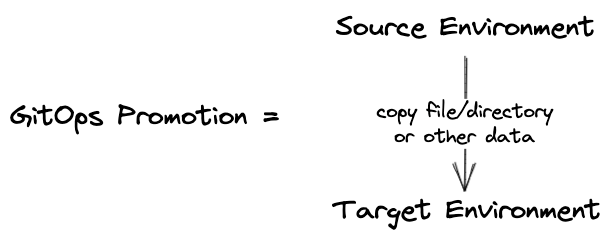
\includegraphics[width=0.60\linewidth]{assets/gitops-promo.png}}
%	\caption{GitOps Promotion.
%		%		(\citeauthor{ref}, \citeyear{ref}).
%	}
%	\label{fig:gitops-promo}	
%\end{figure}

A promotion subject can be potentially many different things.
In the case of this prototype,
a promotion subject is a file or directory,
which is copied from the source to the target environment.
Examples of such files or directories are the following:
\lstinline|kustomization.yaml|,
\lstinline|./component/cert-manager/kustomization.yaml|,
\lstinline|./helm-values-prod.yaml|.
Note, that the relative paths of the promotion subjects,
are relative to the paths of the environment, as defined earlier.

As an example - but outside the scope of the implemented prototype -
a promotion subject could also be fetched from another source,
like an artifact registry, or be any other type of data
and updated/promoted in the target environment,
e.g. a version tag, helm values, etc.

With the proposed and implemented prototype,
the promotion strategy is to raise a pull request at the Git provider
(fig. \ref{fig:raise-pull-request-and-approve}),
with the changes proposed by the promotion.
A human can then review the changes and optionally approve and merge the pull request.
After merging, the promotion will have taken place.

\begin{figure}[h]
	\centering
	\fbox{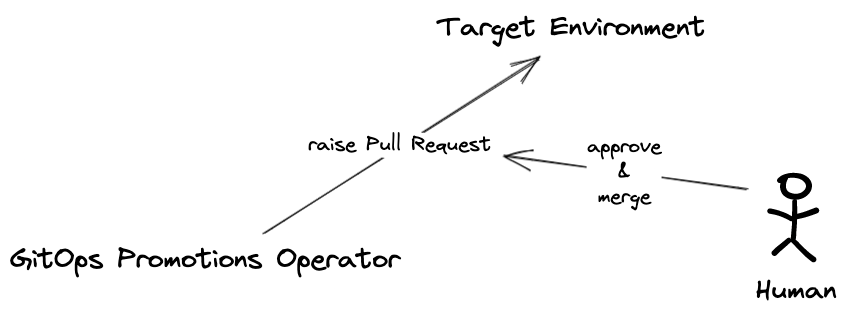
\includegraphics[width=0.98\linewidth]{assets/raise-pull-request-and-approve.png}}
	\caption{Pull Request at target environment.
		%		(\citeauthor{ref}, \citeyear{ref}).
	}
	\label{fig:raise-pull-request-and-approve}	
\end{figure}

Alternatively to a pull request, the changes could be directly
commited and pushed to the target environment,
without human interaction. This strategy should require different means
of automated or otherwise external or additional checks, in order to ensure a safe promotion.
This strategy is not implemented in the developed prototype.

Now that the custom resources are designed,
they need to be implemented.
Since the decision for the prototype is to be developed
with the Kubebuilder framework and follow its style,
mockups of the custom resources in Yaml format
will be created as a next step.









\subsection{Mockups of Custom Resources}
\label{prototype:design:mockups-custom-resources}

%to write mockups
%of custom resources in YAML format,
%since this is what the end user will interface with when the application is finished.
%First and foremost the handling and user experience has to be seamless and make sense
%for the user; also it shouldn't take any extra miles for the user to take,
%just to get started.
%The YAML representation of the custom resource should be similar to other ones
%from the Kubernetes core types.

When the custom resources have been specified,
they can be actually implemented with the framework
as Kubernetes custom resource definitions.

Users will mainly be dealing with the custom resources in a Yaml format.
Yaml keys should be intuitive and make sense to the user.
It also helps if they follow the core Kubernetes definitions regarding naming conventions.
An example for a naming convention is the "Ref" suffix for Yaml keys.
This suffix is typically appended to keys which represent a reference to another Kubernetes
object.
For example, "secretRef" says that this field refers to a Kubernetes secret resource.
A possible mockup for an \textit{Environment} resource
could look like the following.

\lstinputlisting{assets/files/environment-mockup.yaml}

In this mockup the \lstinline|.spec.dependentObjects.workloadRef|
represents a list of Kubernetes objects in the cluster,
which need to be successfully deployed,
before a promotion is triggered.
Additionally the git reference branch main is also specified \\
in the \lstinline|.spec.source.ref.branch| field.

A possible mockup for a GitOps promotion 
could look like the following.

\lstinputlisting{assets/files/promotion-mockup.yaml}

In the promotion mockup definition,
there are four fields in the
\lstinline|.spec|.
These represent the minimum properties of the previously defined abstract definition.
It is to note, that
the \lstinline|.spec.copy| field represents the promotion subjects.
It is a list of items, where each item contains
a \lstinline|name|, \lstinline|source| and \lstinline|target|.
The \lstinline|name| defines a custom name.
The \lstinline|source| and \lstinline|target| fields together define a
file copy operation,
where the \lstinline|source| is the relative path from the source environment,
and the \lstinline|target| is a relative path from the target environment.

\subsection{Alternative Mockups}
\label{prototype:design:alternative-mockups}

The following alternative mockups,
for the custom resource definitions,
i.e. the design of the declarative API,
are suggested, but not implemented in the current prototype.

%\subsubsection*{Promotion Subjects defined in each Environment resource}

Alternatively, the promotion subjects could also be specified
in the environment resource like the following:

\lstinputlisting{assets/files/environment-mockup-alt-1.yaml}

In the promotion definition,
it would then suffice to specify
a list of promotion subjects.

\lstinputlisting{assets/files/promotion-mockup-alt-1.yaml}

This alternative design allows that each environment could have
a unique path of a specific promotion subject defined.
Now if a promotion is spanning over multiple environments,
they could each specify their own unique path to a promotion subject.
The promotion subject is declared in the promotion,
but the actual path is defined per each environment.

\subsection{Translation to Go types}
\label{prototype:design:go-types}

Once the mockups of the custom resources in Yaml format are done,
the declarative structure can be translated to custom Go types.
The full source code of the Go types are found in Appendix \ref{appendix:source-code}.
%The specification of the Environment resource can be seen in Appendix
% \ref{appendix:source-code:environmentSpec-type} \nameref{appendix:source-code:environmentSpec-type}.
%\ref{appendix:source-code}.
The type EnvironmentSpec represents the \lstinline|.spec| Yaml field.
What also needs to be defined is the status subresource.
In the status fields, the controller can save the current/actual state
of the resource during runtime.
While \lstinline|.spec| defines the desired state,
\lstinline|.status| defines the actual state, as observed by the controller.
%The specification of the status resource can be seen in Appendix
% \ref{appendix:source-code:environmentStatusSpec-type} \nameref{appendix:source-code:environmentStatusSpec-type}.
%\ref{appendix:source-code}.
%The specification of the Promotion resource can be seen in Appendix
% \ref{appendix:source-code:promotionSpec-type} \nameref{appendix:source-code:promotionSpec-type}.
%\ref{appendix:source-code}.
For the promotion,
a status subresource is also defined.
In the status - the actual state of the resource as observed by the controller -
most importantly the metadata of the currently opened pull request is saved,
which the controller will pick up on every consecutive reconciliation
of the same promotion object.
%The specification of the status resource can be seen in Appendix
% \ref{appendix:source-code:promotionStatusSpec-type} \nameref{appendix:source-code:promotionStatusSpec-type}.
%\ref{appendix:source-code}.
%The full source code of the types can be found in Appendix
%\ref{appendix:source-code}.
Once the Go types are defined,
the controller logic can be written.

\subsection{Controller Logic}
\label{prototype:design:controller-logic}

In this section,
the controller logic of each implemented control loop, responsible for the according resource,
is described.
This is the controller reconciliation logic which runs on each reconciliation of an object.
The designed logic is prototypical and can change in the future, depending on future requirements
for the \textit{GitOps Promotions Operator}.
% TODO: maybe reference exact section in Appendix of each controller
The full source code of the controllers can be found in Appendix
\ref{appendix:source-code}.


\newpage

\subsubsection*{Environment Controller}

For the environment API,
a controller is written.
For this prototype the following logic is implemented.
It runs on every reconciliation of an environment object from start to finish.
A diagram of the environment controller logic can be seen in figure \ref{tikz:environment-controller-logic}.

\begin{figure}[h]
\centering
\fboxsep6mm\fbox{\begin{tikzpicture}[node distance=1.3cm]
	\node (start) [startstop] {Start};
	\node (dec1) [decision, below of=start, yshift=-1.8cm] {repo is private};
	\node (pro1a) [process, right of=dec1, xshift=4cm] {configure auth};
	\node (pro1) [process, below of=dec1, yshift=-1.8cm] {test clone};
	\node (out1) [process, below of=pro1] {mark as available};
	\node (stop) [startstop, below of=out1] {Stop};
	
	\draw [arrow] (start) -- (dec1);
	\draw [arrow] (dec1) -- node[anchor=east] {yes} (pro1a);
	\draw [arrow] (dec1) -- node[anchor=south] {no} (pro1);
	\draw [arrow] (pro1a) |- (pro1);
	\draw [arrow] (pro1) -- (out1);
	\draw [arrow] (out1) -- (stop);
\end{tikzpicture}}
\caption{Environment Controller Logic.} \label{tikz:environment-controller-logic}
\end{figure}

At first, it is checked if the respective source Git repository
of the environment object is private.
If it is private,
additional authentication options are configured,
in order to be able to access the private Git repository.
If it is publicly accessible, there is no need to configure authentication.
Next, a Git clone process is tested for the environment.
It is cloned locally, but afterwards disregarded.
When it succeeds,
the environment object is marked as available.
This is achieved by updating the object's status.
The status is observable by other controllers, like the promotion controller.
This prototypical controller logic for the environment controller
may be extended for additional functionality in the future.

%\begin{tikzpicture}[node distance=2cm]
%	
%	\node (start) [startstop] {Start};
%	\node (in1) [io, below of=start] {Input};
%	\node (pro1) [process, below of=in1] {Process 1};
%	\node (dec1) [decision, below of=pro1, yshift=-0.5cm] {Decision 1};
%	
%	\node (pro2a) [process, below of=dec1, yshift=-0.5cm] {Process 2a
%		text text text text
%		text text text 
%		text text text};
%	
%	\node (pro2b) [process, right of=dec1, xshift=2cm] {Process 2b};
%	\node (out1) [io, below of=pro2a] {Output};
%	\node (stop) [startstop, below of=out1] {Stop};
%	
%	\draw [arrow] (start) -- (in1);
%	\draw [arrow] (in1) -- (pro1);
%	\draw [arrow] (pro1) -- (dec1);
%	\draw [arrow] (dec1) -- node[anchor=east] {yes} (pro2a);
%	\draw [arrow] (dec1) -- node[anchor=south] {no} (pro2b);
%	\draw [arrow] (pro2b) |- (pro1);
%	\draw [arrow] (pro2a) -- (out1);
%	\draw [arrow] (out1) -- (stop);
%	
%\end{tikzpicture}


\newpage

\subsubsection*{Promotion Controller}

For the promotion API,
the following controller logic is implemented.
It runs on every reconciliation of an environment object from start to finish.
A diagram of the promotion controller logic can be seen in figure \ref{tikz:promotion-controller-logic}.

\begin{figure}[h]
	\centering
	\fboxsep6mm\fbox{\begin{tikzpicture}[node distance=1.3cm]
		\node (start) [startstop] {Start};
		\node (in1) [process, below of=start] {ensure environments are available};
		\node (proClone) [process, below of=in1] {clone repos};
		\node (proCheckPending) [process, below of=proClone] {check pending promotion};
		\node (proExecProm) [process, below of=proCheckPending] {execute promotion operations};
		\node (dec1) [decision, below of=proExecProm, yshift=-1.8cm,text width=3cm] {source != target environment};
		\node (pro1a) [process, right of=dec1, xshift=4cm] {push PR branch};
		\node (pro1) [process, below of=dec1, yshift=-1.8cm] {create/update PR};
		\node (out1) [process, below of=pro1] {mark as ready};
		\node (stop) [startstop, below of=out1] {Stop};
		
		\draw [arrow] (start) -- (in1);
		\draw [arrow] (in1) -- (proClone);
		\draw [arrow] (proClone) -- (proCheckPending);
		\draw [arrow] (proCheckPending) -- (proExecProm);
		\draw [arrow] (proExecProm) -- (dec1);
		\draw [arrow] (dec1) -- node[anchor=east] {yes} (pro1a);
		\draw [arrow] (dec1) -- node[anchor=south] {no} (pro1);
		\draw [arrow] (pro1a) |- (pro1);
		\draw [arrow] (pro1) -- (out1);
		\draw [arrow] (out1) -- (stop);
	\end{tikzpicture}}
	\caption{Promotion Controller Logic.} \label{tikz:promotion-controller-logic}
\end{figure}

The controller checks if the source and target environments are ready,
this includes the check of their defined dependent objects.
If they are not yet ready, the controller cancels the reconciliation immediately.
Then the source and target environments are cloned.
Next the controller checks if there is a pending/open pull request,
this information is retrieved from the object's status, and then checked
if still up to date via the Git provider's API.
Afterwards the controller executes the promotion operations.
%which are the copy operations with the current state of the prototype.
If there were changes since the last reconciliation, the new commits
are pushed to the pull request branch.
Then a pull request will be raised, if not yet done during a previous reconciliation.
Lastly, the promotion is marked as ready in its status.















\section{Demonstration}
\label{prototype:demonstration}

The following section demonstrates the in-context usage of the
developed prototype - the \textit{GitOps Promotions Operator} - in a proof of concept.
The use case described as follows is created for the purpose of this demonstration.

This use case deals with a setup with multiple deployment environments.
There are two non-critical environments \lstinline|dev| and \lstinline|qa|,
and two production environments \lstinline|prod-1| and \lstinline|prod-2|.
The GitOps definitions of the non-critical environments are living inside the same
Git repository \lstinline|mtpoc-infra-1|,
and each production environment lives in its own separate Git repository
\lstinline|mtpoc-infra-2| for \lstinline|prod-1|,
and \lstinline|mtpoc-infra-3| for \lstinline|prod-2|.
In general, the application version shall be promoted with a strict flow
through the environments, one after the other.
An overview of the given setup can be seen in the table \ref{table:poc-environments-setup}.

\begin{table}[h]
\begin{center}
	\begin{tabular}{||c c c||} 
		\hline
		Order & Environment & Source Repository \\ [0.5ex] 
		\hline\hline
		1 & dev & mtpoc-infra-1 \\ 
		\hline
		2 & qa & mtpoc-infra-1 \\
		\hline
		3 & prod-1 & mtpoc-infra-2 \\
		\hline
		4 & prod-2 & mtpoc-infra-3 \\
%		[1ex]
		\hline
	\end{tabular}
	\caption{PoC Environments Setup}
	\label{table:poc-environments-setup}
\end{center}
\end{table}

The GitOps environment is centered around the used configuration management tool
Kustomize, and generally structured for all environments as below:

\begin{lstlisting}
.
|-- app-version
|   `-- kustomization.yaml
|-- kustomization.yaml
`-- settings
    `-- deployment.yaml
\end{lstlisting}

However it is independent of the tool Kustomize;
any other tools can be used in conjunction with the proposed operator prototype.
This structure adheres to the constraints of the currently implemented
copy operation promotion type, which can copy files and directories.
This means the configuration components which need to be promoted,
should be defined in separate files or directories.
This is needed, in order to only promote e.g. the application image version,
while leaving other configuration untouched, and specific to an environment.
With the Kustomize configuration tool, it is possible to split
parts of the main \lstinline|kustomization.yaml| into other separated files,
with the components feature.

In this use case, the value of the application's image version lives within the 
app-version component. This is configured in the main \lstinline|kustomization.yaml|
like this:

\begin{lstlisting}
components:
- app-version
\end{lstlisting}

The \lstinline|./app-version| directory contains a \lstinline|kustomization.yaml| file,
with typical Kustomization specification.
In this case, the images feature of Kustomize is used for configuring the application's
image version tag.

\begin{lstlisting}
apiVersion: kustomize.config.k8s.io/v1alpha1
kind: Component
images:
- name: ghcr.io/stefanprodan/podinfo
newTag: 6.3.4
\end{lstlisting}

Now the goal is to configure a promotion for the app-version component.
To achieve this, 
an \lstinline|Environment| resource needs to be created
for all environments respectively.
Only the \lstinline|dev| environment is shown here,
the other three environment definitions follow the same schema,
but are omitted from this demonstration for the sake of brevity.

\lstinputlisting{assets/files/dev-environment.yaml}

%\lstinputlisting{assets/files/qa-environment.yaml}
%
%\lstinputlisting{assets/files/prod-1-environment.yaml}
%
%\lstinputlisting{assets/files/prod-2-environment.yaml}

Now the specified secrets must be created.
The API token is required for the creation of pull requests by the promotion controller;
it must be stored in a Kubernetes generic secret resource in a key named \lstinline|token|,
and can be created with the following command:

\lstinline|kubectl create secret generic github-api-token --from-literal=token="gh..."|

With the current prototype, also a secret for the SSH connection to push and pull
the repository, needs to be created.
For this, a ssh key pair needs to be created by the user. Its public key needs to 
be set as a deploy key at the Git provider,
and its private key needs to be stored in a
Kubernetes generic secret resource in a key named \lstinline|private|.

\lstinline|kubectl create secret generic github-api-token --from-literal=private="--..."|

When all the four environments are created, the \lstinline|Promotion| resources
can be defined.
In this use case, three promotion resources are needed for the ability to
promote between all four environments with a straight flow - promoting from one to the next.
Only the \lstinline|dev-to-qa| promotion is shown here,
the other two definitions follow the same schema,
but are omitted here for the sake of brevity.

\lstinputlisting{assets/files/dev-to-qa.yaml}

%\lstinputlisting{assets/files/qa-to-prod-1.yaml}
%
%\lstinputlisting{assets/files/prod-1-to-prod-2.yaml}





At this point, all which is needed for promoting is configured.
When the status of all the environment resources involved in a promotion,
have a ready status condition,
and the dependent objects are successfully deployed,
a promotion will trigger.
%\lstinputlisting{assets/files/env-dev-status.yaml}
At this point, the controller logs can be observed.

\begin{lstlisting}
2023-04-16T12:10:46Z INFO    Created new pull request    [...]
\end{lstlisting}
%2023-04-16T12:10:40Z    INFO    Begin reconciling Promotion     {"controller": "promotion", "controllerGroup": "promotions.gitopsprom.io", "controllerKind": "Promotion", "Promotion": {"name":"dev-to-qa","namespace":"default"}, "namespace": "default", "name": "dev-to-qa", "reconcileID": "ba3775ae-d8b1-40de-ad7b-4f42f8534686", "name": {"namespace": "default", "name": "dev-to-qa"}}
%2023-04-16T12:10:46Z    INFO    Created new pull request        {"controller": "promotion", "controllerGroup": "promotions.gitopsprom.io", "controllerKind": "Promotion", "Promotion": {"name":"dev-to-qa","namespace":"default"}, "namespace": "default", "name": "dev-to-qa", "reconcileID": "ba3775ae-d8b1-40de-ad7b-4f42f8534686", "WebURL": "https://github.com/thomasstxyz/mtpoc-infra-1/pull/1"}
%2023-04-16T12:10:46Z    INFO    Reconciled Promotion successfully       {"controller": "promotion", "controllerGroup": "promotions.gitopsprom.io", "controllerKind": "Promotion", "Promotion": {"name":"dev-to-qa","namespace":"default"}, "namespace": "default", "name": "dev-to-qa", "reconcileID": "ba3775ae-d8b1-40de-ad7b-4f42f8534686", "duration": "6.050374419s", "nextReconcile": "300s"}

A new pull request
%with the number \lstinline|1|
%at the Web URL \\
%\url{https://github.com/thomasstxyz/mtpoc-infra-1/pull/1} \\
has been created by the controller.
The promotion's status will also reflect, that
a pull request is open for review.

\lstinputlisting{assets/files/prom-dev-to-qa-status.yaml}

The open pull request is ready for review in the Git provider's web interface.
%%\begin{figure}[h]
%%	\centering
%%	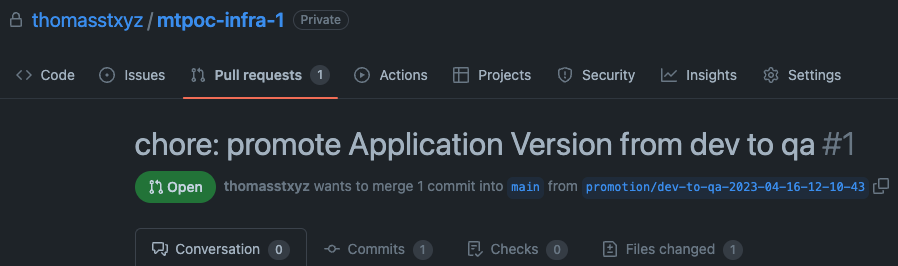
\includegraphics[width=1.00\linewidth]{assets/new-promotion-github.png}
%%	\caption{New Git Pull Request.
%%		%		(\citeauthor{ref}, \citeyear{ref}).
%%	}
%%	\label{fig:new-promotion-github}	
%%\end{figure}
\begin{figure}[h]
	\centering
	\fboxsep0mm\fbox{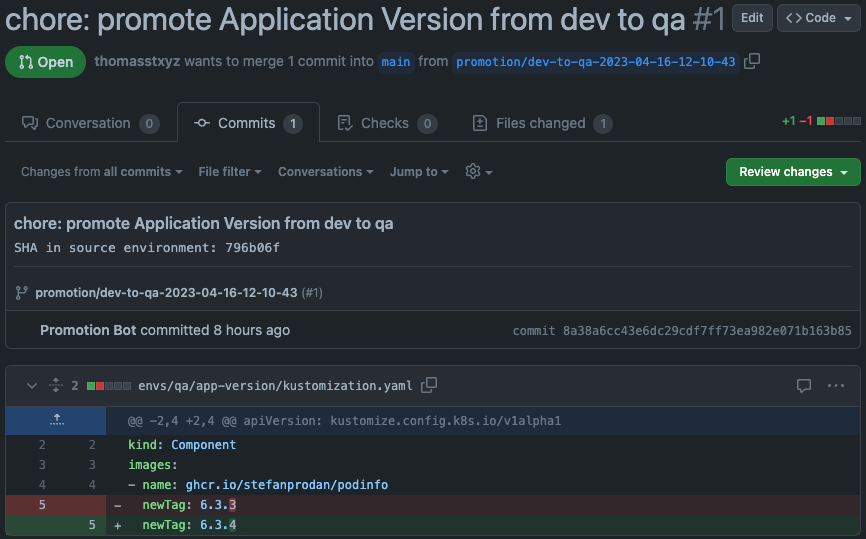
\includegraphics[width=0.98\linewidth]{assets/prom-pr-dev-to-qa.png}}
	\caption{Pull Request for Promotion from dev to qa.
		%		(\citeauthor{ref}, \citeyear{ref}).
	}
	\label{fig:prom-pr-dev-to-qa}	
\end{figure}

The changed difference introduced by the commit can be viewed:

\begin{lstlisting}
- newTag: 6.3.3
+ newTag: 6.3.4
\end{lstlisting}

The \lstinline|dev-to-qa| promotion requested the change of the image version from
\lstinline|6.3.3| to \lstinline|6.3.4|.

Now, since the \lstinline|qa| and the \lstinline|prod-1| environments
also differ,
a pull request has also been created for this promotion.

%\begin{figure}[h]
%	\centering
%	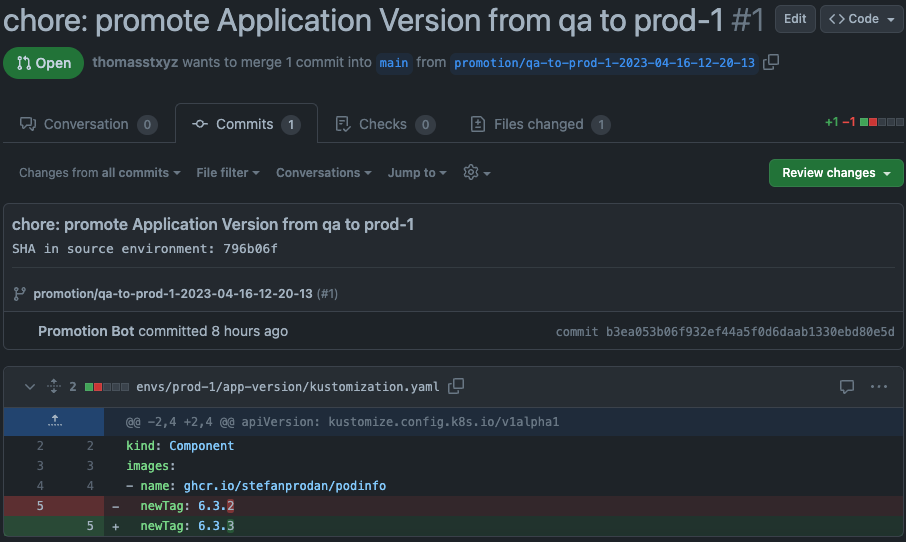
\includegraphics[width=1.00\linewidth]{assets/prom-pr-qa-to-prod-1.png}
%	\caption{Pull Request for Promotion from qa to prod-1.
%		%		(\citeauthor{ref}, \citeyear{ref}).
%	}
%	\label{fig:prom-pr-qa-to-prod-1}	
%\end{figure}

The \lstinline|qa-to-prod-1| promotion requested the change of the image version from
\lstinline|6.3.2| to \lstinline|6.3.3|.

\begin{lstlisting}
- newTag: 6.3.2
+ newTag: 6.3.3
\end{lstlisting}

Since the \lstinline|prod-1| and the \lstinline|prod-2| environments
now also differ,
a pull request has also been created for this promotion.

%\begin{figure}[h]
%	\centering
%	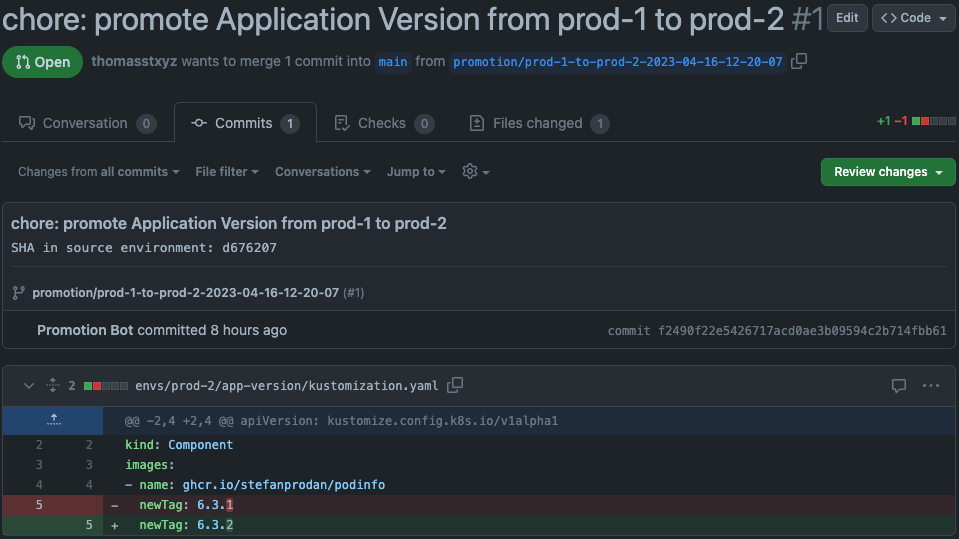
\includegraphics[width=1.00\linewidth]{assets/prom-pr-prod-1-to-prod-2.png}
%	\caption{Pull Request for Promotion from prod-1 to prod-2.
%		%		(\citeauthor{ref}, \citeyear{ref}).
%	}
%	\label{fig:prom-pr-prod-1-to-prod-2}	
%\end{figure}

The \lstinline|prod-1-to-prod-2| promotion requested the change of the image version from
\lstinline|6.3.1| to \lstinline|6.3.2|.

\begin{lstlisting}
- newTag: 6.3.1
+ newTag: 6.3.2
\end{lstlisting}

If the \lstinline|dev| environment advances the application image version further,
the pull request for the \lstinline|dev-to-qa| will be updated with another commit.
Note that the previous commit is not overwritten, 
but the commit history is kept on the pull request branch - now there are two commits on the branch.

\begin{figure}[h]
	\centering
	\fboxsep0mm\fbox{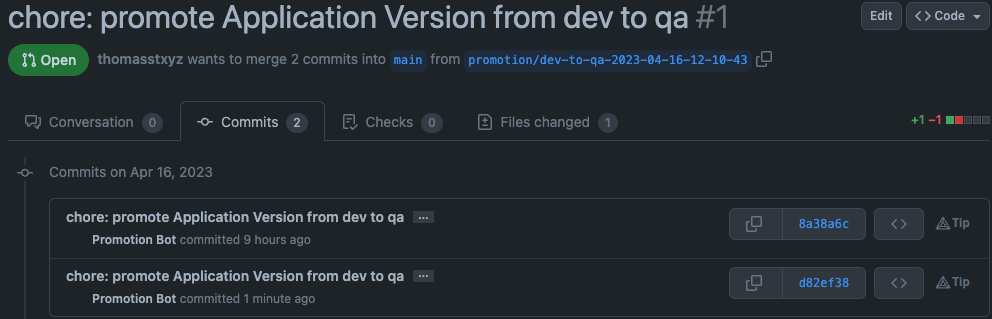
\includegraphics[width=0.98\linewidth]{assets/prom-pr-dev-to-qa-round2.png}}
	\caption{Pull Request updated for Promotion from dev to qa.
		%		(\citeauthor{ref}, \citeyear{ref}).
	}
	\label{fig:prom-pr-dev-to-qa-round2}	
\end{figure}

The difference for the \lstinline|dev-to-qa| promotion is now:

\begin{lstlisting}
- newTag: 6.3.3
+ newTag: 6.3.5
\end{lstlisting}

%\begin{figure}[h]
%	\centering
%	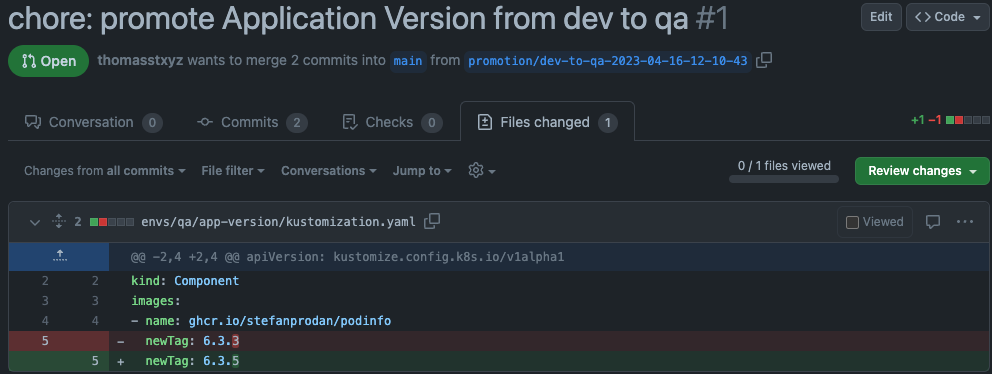
\includegraphics[width=1.00\linewidth]{assets/prom-pr-dev-to-qa-round2-diff.png}
%	\caption{Pull Request updated for Promotion from dev to qa (diff).
%		%		(\citeauthor{ref}, \citeyear{ref}).
%	}
%	\label{fig:prom-pr-dev-to-qa-round2-diff}	
%\end{figure}

Now if the pull request for the \lstinline|dev-to-qa| promotion
is approved and merged by a human,
the promotion will actually take effect.
This results in the \lstinline|qa-to-prod-1| promotion pull request being updated
by the promotion controller.
Version \lstinline|6.3.5| is now requested for promotion to the
\lstinline|prod-1| environment.

The difference for the \lstinline|qa-to-prod-1| promotion is now:

\begin{lstlisting}
- newTag: 6.3.2
+ newTag: 6.3.5
\end{lstlisting}

Once reviewed, approved and merged by a human,
the promotion of version \lstinline|6.3.5| to the \lstinline|prod-1| environment
will result in further propagation of version \lstinline|6.3.5|
to the \lstinline|prod-2| environment.

The difference for the \lstinline|prod-1-to-prod-2| promotion pull request is now:

\begin{lstlisting}
- newTag: 6.3.1
+ newTag: 6.3.5
\end{lstlisting}

Once reviewed, approved and merged by a human,
the promotion of version \lstinline|6.3.5| to the \lstinline|prod-2| environment
will take effect.

The described demonstration showed,
how an application version can be promoted across multiple environments,
while ensuring a strict flow of promotion of \\
e.g. \lstinline|dev --> qa --> prod-1 --> prod-2|.
Alongside the application version or any arbitrary resource,
users of the prototype operator may specify multiple other
promotion subjects in the copy operations list \lstinline|.spec.copy|, which shall be promoted.
For the sake of brevity, this was not shown in detail in the demonstration.





%For this demonstration, it is supposed that
%the latest version \lstinline|6.3.5| is bad and should not be promoted,
%instead the \lstinline|dev| environment shall be rolled back to \lstinline|6.3.4|.






















\section{Evaluation}
\label{prototype:evaluation}

Now that the prototype has been demonstrated in a proof of concept,
its functionality is compared against the solution objectives,
as defined in section
\ref{interviews:definitionSolutionObjectives}
earlier in this thesis.
The evalutation is achieved by means of
comparing the qualitative descriptions of the solution objectives against the
observed functionality of the prototype in the demonstration in section \ref{prototype:demonstration}.

\subsection*{Objective 1}

The requirement 1 of objective 1 (OBJ1R1), formulated as a user story,
was the following:

\begin{quotation}
	\noindent
	\ref{OBJ1R1}
\end{quotation}

As demonstrated in section
\ref{prototype:demonstration}
the user of the \textit{GitOps Promotions Operator} can define promotion subjects
in the form of file/directory copy operations inside the Promotion custom resource.
The source and target may be in separate Git repositories, respective \textit{Environment} custom resources.
This creates the possibility to promote arbitrary resources.
The demonstration shows a promotion of the "Application Version",
which is actually a specified file kustomization.yaml with a Kustomize component,
which sets a new image tag.
The defined name of the arbitrary filesystem path serves as the demonstration for the requirement 2 (OBJ1R2).

\begin{quotation}
	\noindent
	\ref{OBJ1R2}
\end{quotation}

The definition of such a descriptive name helps to identify promotion subjects more easily, especially when
they are arbitrary files or directories. The name can be represented in the commit message or pull request, as demonstrated.

\subsection*{Objective 2}

The requirement 1 of objective 2 (OBJ2R1) was the following:

\begin{quotation}
	\noindent
	\ref{OBJ2R1}
\end{quotation}

The prototypical implementation of the functionality of the solution objective is demonstrated in section
\ref{prototype:demonstration}.
It is shown, how a new application release can be promoted through multiple environments in a specified order.
After deployment to the \lstinline|dev| environment, a promotion is requested for the \lstinline|qa| environment.
Once a human has approved and merged the pull request, the promotion to \lstinline|qa| takes its effect.
Afterwards the promotion from \lstinline|qa| to \lstinline|prod-1| environment is requested. Upon successful promotion to \lstinline|prod-1|,
the release is finally promoted from \lstinline|prod-1| to \lstinline|prod-2|.

\subsection*{Objective 3}

The requirement 1 of objective 3 (OBJ3R1) was the following:

\begin{quotation}
	\noindent
	\ref{OBJ3R1}
\end{quotation}

The functionality of this objective is demonstrated in context in the proof of concept
in section \ref{prototype:demonstration}.
In the \lstinline|Environment| custom resource,
a field
\lstinline|dependentObjects.workloadRef| may be defined, under which a user can specify
a list of Kubernetes workloads of the kind Deployment.
The developed prototype supports object types of kind Deployment,
however, any Kubernetes native resource, as well as custom resource, can potentially be added as an
additional feature for the prototype.
For example, a field \lstinline|dependentObjects.externalHttpRef| could be added,
with the logic for calling HTTP/S URIs, and parsing the result.

\subsection*{Objective 4}

The requirement 1 of objective 4 (OBJ4R1) was the following:

\begin{quotation}
	\noindent
	\ref{OBJ4R1}
\end{quotation}

The developed prototype \textit{GitOps Promotions Operator} supports the use of GitHub currently,
however the custom resource API is designed with a generic specification and therefore allows
for adding the support for any other Git provider in the future.
The same vendor-neutral approach was chosen for the GitOps engine.
%These are most often from the Flux or Argo projects.
The \textit{GitOps Promotions Operator} prototype allows the use of any GitOps engine,
because it interfaces only with Kubernetes built-in resources.
Furthermore, the prototype is agnostic to the configuration/templating tool which may be used or not.
%This is most prominently Helm and Kustomize.
Since the operator provides the ability
to promote arbitrary files or directories in Git repositories, it is not needed to specifically integrate
with the named tools.






\section{Summary}

In this preceding chapter,
the proposed prototype was presented.
The asynchronous nature of GitOps deployments, and where
the operator prototype fits within this architecture was described.
Next, abstract models for the \textit{Environment} and \textit{Promotion} custom resources as well as their prototype
design as declarative Kubernetes custom resources was described.
The implementation of these custom resources was shown in the form of mockups
of Kubernetes custom resources in the Yaml format.
Alternative mockup designs were shown as a way to draw attention to the fact
that the actual design of the API specification may be changed as desired.
%Moreover, the API specification should be tested with users,
%and should be adapted for usability and ease of use.
The translation of the API specification in Yaml format into Go types was described,
and finally the implemented controller reconciliation logic of both the environment, as well as
the promotion controller was presented.

In the next step, the developed artifact of the prototype operator was
demonstrated in the context of a proof-of-concept use case.
The demonstration of the prototype's functionality was then evaluated against
the research objectives defined in
\ref{interviews:definitionSolutionObjectives}.














%\chapter{Interviews with Working Professionals}
%
%\section{Categorisation of Findings}
%\section{Common Problem Definitions}
%\section{...?}
%
%
%\chapter{Definition of Solution Objectives}
%
%\section{People \& Communication Perspective}
%\section{Technical Perspective}
%\section{...?}
%
%
%\chapter{Prototype Design and Development}
%
%\section{Architecture}
%\section{Functionality}
%\section{...?}
%
%\chapter{Proof-of-Concept Demonstration}
%
%\section{Setup and Use with Kustomize}
%\section{Setup and Use with Helm}
%\section{Multiple Environments in same Stage}
%\section{Scalability}
%\section{...?}















%
%\section{Instruction included in the original FHBgld word processor template}
%Die Durchführung der empirischen Untersuchung ist nachvollziehbar zu dokumentieren sowie auch die dabei aufgetretenen Probleme und deren Behandlung. Der Umfang ergibt sich aus der Art der Bearbeitung.  
%
%Tabelle 1 zeigt ein Bespiel für eine Tabelle. 
%
%\begin{figure}[ht]
%	\centering
%	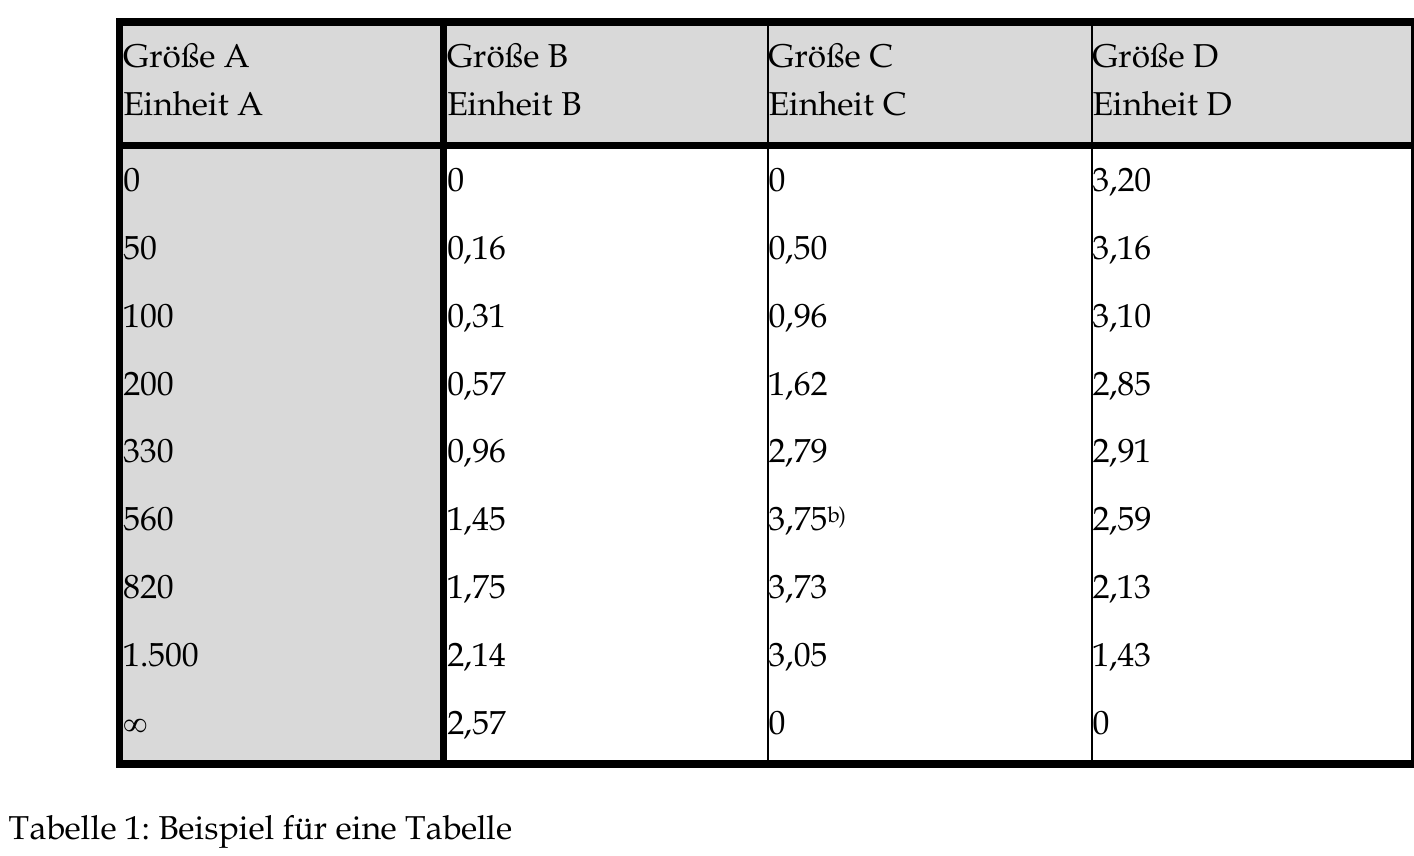
\includegraphics[width=0.7\linewidth]{figures/Word_Table}
%	\caption{Screenshot example from FHBgld word processor template}
%	\label{fig:wordtable}
%\end{figure}
%Abbildung 1 zeigt ein Beispiel für eine Abbildung oder Grafik.
%\begin{figure}
%	\centering
%	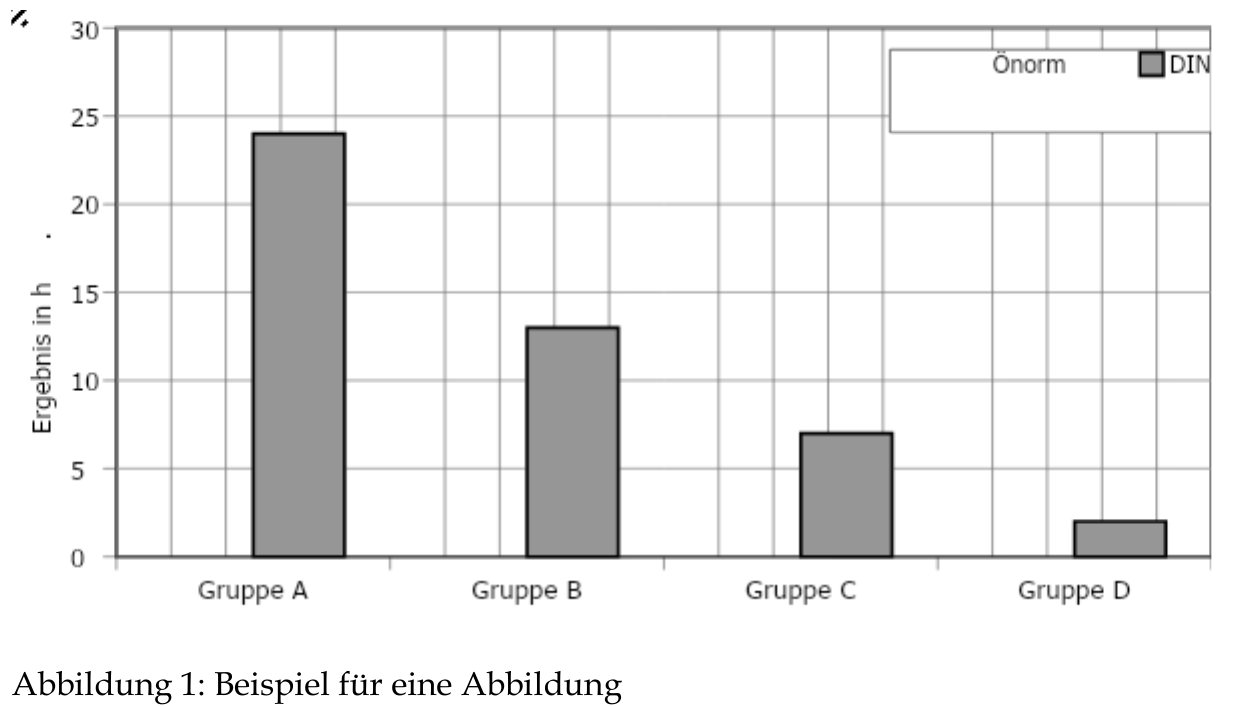
\includegraphics[width=0.7\linewidth]{figures/Word_Diagram}
%	\caption{Screenshot example from FHBgld word processor template}
%	\label{fig:worddiagram}
%\end{figure}
%\linebreak
%Mathematisch werden die Zusammenhänge wie im Figure \ref{fig:wordformel} beschrieben.
%\begin{figure}
%	\centering
%	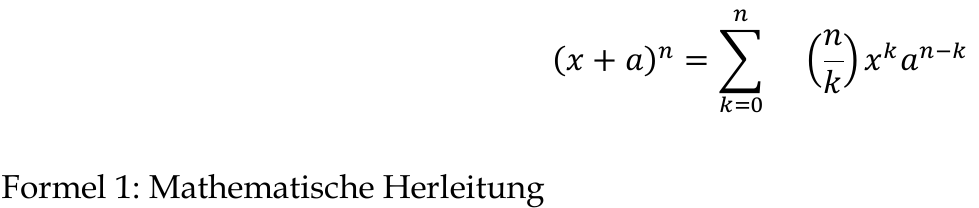
\includegraphics[width=0.7\linewidth]{figures/Word_Formel}
%	\caption{Screenshot example from FHBgld word processor template}
%	\label{fig:wordformel}
%\end{figure}
%
%\section{Tables and Images with \LaTeX}
%One of the great advantages of \LaTeX{} is that all it needs to know is
%the structure of a document, and then it will take care of the layout
%and presentation itself.  So, here we shall begin looking at how exactly
%you tell \LaTeX{} what it needs to know about your document.
%
%\subsection{Tables}
%In this sub-section, a simple table is inserted. To add reference to the table, see (cf. Table~\hyperref[tab:tableexample0]{\ref{tab:tableexample0}}):
%
%%A simple table.  The center environment is first set up, otherwise the
%%table is left aligned.  The tabular environment is what tells Latex
%%that the data within is data for the table.
%% https://en.wikibooks.org/wiki/LaTeX/Tables
%\begin{table}[htb]
%	\begin{tabular}{|b{7cm}|c|}
%		%The tabular environment is what tells Latex that the data within is
%		%data for the table.  The arguments say that there will be two
%		%columns, both left justified (indicated by the 'l', you could also
%		%have 'c' or 'r'.  The bars '|' indicate vertical lines throughout
%		%the table.
%		
%		\hline  % Print horizontal line
%		\fontsize{11pt}{12pt}\selectfont Command & Level \\ \hline  % Columns are delimited by '&'.  And
%		%rows are delimited by '\\'
%		\fontsize{10pt}{14pt}\selectfont Some sections to provide some examples: & \\
%		\texttt{\textbackslash part\{\emph{part}\}} & -1 \\
%		\texttt{\textbackslash chapter\{\emph{chapter}\}} & 0 \\
%		\texttt{\textbackslash section\{\emph{section}\}} & 1 \\
%		\texttt{\textbackslash subsection\{\emph{subsection}\}} & 2 \\
%		\texttt{\textbackslash subsubsection\{\emph{subsubsection}\}} & 3 \\
%		\texttt{\textbackslash paragraph\{\emph{paragraph}\}} & 4 \\
%		\texttt{\textbackslash subparagraph\{\emph{subparagraph}\}} & 5 \\
%		\hline
%		
%	\end{tabular}
%	\caption{some description of the table}
%	\label{tab:tableexample0}
%\end{table}
%
%\subsubsection{More tabular examples}
%
%First, a plain simple example for a FHBgld table, see table~\hyperref[tab:tab:tableexample1]{\ref{tab:tableexample1}}.
%
%\begin{table}[h]
%	\centering
%	\begin{tabular}{|b{1cm}|b{2cm}|b{3cm}|b{4cm}|}
%		\hline
%		\multicolumn{4}{|l|}{\fontsize{11pt}{12pt}\selectfont\noindent First line in 11pt fontsize } \\ \hline
%		1cm & 2cm & 3cm & 4cm \\ \hline
%		from & here on & the table & font size \\ \hline
%		will & be as & defined & in class, that is 10pt\footnote{yes, really!} \\ \hline
%		will & be as & defined & in class, that is 10pt\footnote{yes, really!} \\ \hline
%		will & be as & defined & in class, that is 10pt\footnote{yes, really!} \\ \hline
%		will & be as & defined & in class, that is 10pt\footnote{yes, really!} \\ \hline
%		will & be as & defined & in class, that is 10pt\footnote{yes, really!} \\ \hline
%	\end{tabular}
%	\caption{some description of the table}
%\label{tab:tableexample1}
%\end{table}
%
%Next, a table with nine columns, see table~\hyperref[tab:tableexample2]{\ref{tab:tableexample2}}.
%
%\begin{table}[h]
%	\centering
%	\begin{tabular}{|*{9}{l|}}
%		\hline
%		{\fontsize{11pt}{12pt}\selectfont This} & {\fontsize{11pt}{12pt}\selectfont table} & {\fontsize{11pt}{12pt}\selectfont has} & {\fontsize{11pt}{12pt}\selectfont way} & {\fontsize{11pt}{12pt}\selectfont too } & {\fontsize{11pt}{12pt}\selectfont many} & {\fontsize{11pt}{12pt}\selectfont columns}, & {\fontsize{11pt}{12pt}\selectfont does'nt} & {\fontsize{11pt}{12pt}\selectfont it?} \\ \hline
%		One & Two & Three & Four & Five & Six & Seven & Eight & Nine! \\ \hline
%		At & least & the & first & column & has & 11pt & font & size. \\ \hline
%	\end{tabular}
%	\caption{some description of the table}
%	\label{tab:tableexample2}
%\end{table}
%
%\subsection{Images}
%% Here is how to insert an image as a figure. There is a lot more you can do
%% when inserting images, check out: https://en.wikibooks.org/wiki/LaTeX/Importing_Graphics
%
%\begin{figure}[h]
%	\centering
%	
\includegraphics[width=0.3\textwidth]{figures/logo_nontransparent.jpg}
%	\caption{Image Example}
%	\label{fig:image_example}
%\end{figure}
%
%When an image is inserted, you can refer to it like this (cf. Figure~\hyperref[fig:image_example]{\ref{fig:image_example}}).
%
%\subsubsection{A Subsubsection}
%As one last example, this is how you can insert a sub-sub-section! Have fun
%writing your thesis with \LaTeX{}!
%
%\lipsum[2-3]
%\raggedbottom
%
%\pagebreak
